\documentclass[5p]{elsarticle}

\usepackage{lineno,hyperref}
\usepackage{graphicx}
\usepackage{url}
\usepackage{subfig}
\usepackage{amsmath}
\usepackage{algorithm}
\usepackage{algpseudocode}
\usepackage{booktabs}
\modulolinenumbers[5]

\journal{Journal of Neural Networks}

\bibliographystyle{bst/elsarticle-num}

\begin{document}

\begin{frontmatter}

\title{V4 Neural Network Model for Shape-based Feature Extraction and Object Discrimination}

\author{Zheng Dong}
\ead{dongzheng@fudan.edu.cn}

\author{Hui Wei\corref{cor:1}}
\cortext[cor:1]{Corresponding author}
\ead{weihui@fudan.edu.cn}

\address{Laboratory of Cognitive Modeling and Algorithms, %
School of Computer Science, Fudan University, Shanghai, China}

\begin{abstract}
This template helps you to create a properly formatted \LaTeX\ manuscript.
\end{abstract}

\begin{keyword}
\texttt{elsarticle.cls}\sep \LaTeX\sep Elsevier \sep template
\MSC[2010] 00-01\sep  99-00
\end{keyword}

\end{frontmatter}

\linenumbers

\section{Introduction}

Understanding the content of images has always been a difficult task in image analysis
due to the well known semantic gap \cite{smeulders2000}.
A high degree of abstraction is required to transform low-level pixel data into high-level knowledge of the images.
Computer vision researchers attempt to bridge the gap between pixel data and image content with image features.
Various methods have been proposed to extract features from pixel representation of images.
However, humans and primates outperform any existing computer vision system with respect to almost any measure.
How visual cortex recognizes objects is a critical question for neuroscience.
Visual stimuli captured by the eye are transformed into neural impulses in the retina and further processed by 
the visual cortex for high level cognitive tasks.
The visual cortex plays an important role in filling the gap
between visual stimuli and the implied semantic information.
Neural impulses travel through the visual pathway \cite{ettlinger1990}
in the visual cortex and finally contribute to a unified percept of the object of interest. 

Primate brains possess two distinct visual pathways \cite{ettlinger1990,lehky2007}.
The dorsal pathway is involved with processing the object's spatial location relevant to the viewer. 
The ventral pathway is involved with object discrimination and recognition.
In this paper, we concentrate on the latter, the ventral pathway, and visual area V4 in particular.
V4 lies in the middle of the ventral pathway (\figurename~\ref{fig:1}).
Lower levels of the pathway (visual areas V1 and V2) extract preliminary visual features 
including edges and orientations \cite{hubel1962,hubel1965}.
Higher levels of the pathway (inferior temporal cortex) exhibit selectivity to complex objects
like faces and body parts \cite{bruce1981,bell2009}.
As an intermediate stage, V4 plays a crucial role in transforming low-level orientation signals 
into complex object representations.

\begin{figure}
\centerline{\includegraphics[width=0.8\linewidth]{images/fig-1.png}} 
\caption{V4 is an intermediate stage in visual recognition.}
\label{fig:1}
\end{figure}

In this paper, we propose a multi-layer neural network model
which imitates the neural mechanism of visual area V4 in the ventral visual pathway.
Different stages of the neural pathway in the visual cortex
are explicitly mapped to different layers of the neural network model.
In this feed-forward network, features are extracted hierarchically from input images. 
High-level local image features emerge in the output layer of the network. 
The features encode local structures of object shapes in a way which closely resembles the mechanism of the cortex 
and therefore achieve a good balance between the discrimination and generalization abilities.
The features exhibit competitive performance when applied to object recognition tasks.
Moreover, this multilayer neural network shows a successful attempt 
to integrate different stages of visual processing in the brain. 
It provides an extensible framework so that future findings in cortex mechanisms 
can be adopted and applied to computer vision tasks.

We briefly introduce some related work on traditional image features
and the biological background of our model in section~\ref{sec:2}.
We focus on the shape selectivity of area V4 and some previous models of V4 are also discussed in this section.
In section~\ref{sec:3}, we give the detailed description of our proposed model.
It is capable of locating salient points 
and generating discriminative local shape features around each salient point.
In section~\ref{sec:4}, empirical evaluation shows that
the model demonstrates similar selectivity compared with V4 neurons.
and compared with other models in section~\ref{sec:exp}. 
The conclusion is summarized in section~\ref{sec:conclusion}.

\section{Related work}\label{sec:2}

\subsection{Traditional image features}

Image features encode the image structure in a spatial neighborhood around each of a set of interest points.
Extracting features is an important stage in the process of understanding the content of an image.
These features can be low-level features, such as edges \cite{canny1986} 
and corners \cite{harris1988,smith1997},
or high-level features, which are usually more distinctive and descriptive.

Traditional image features mostly fall into three categories \cite{mikolajczyk2005}: 
distribution-based descriptors, spatial-frequency descriptors and differential-based descriptors.
Distribution-based descriptors use histograms 
to represent characteristics of local image regions.
SIFT descriptor \cite{lowe1999} (including its variations) 
and shape context \cite{belongie2002} are typical examples of such descriptors.
SIFT descriptor uses histograms 
of oriented image gradients over rectangular grids.
Shape context implements similar idea 
by computing histograms of edge pixels in a log-polar grid.
Spatial-frequency descriptors and differential-based descriptors 
use filters and derivatives to capture the invariant features. 
Examples of these categories are 
complex filters \cite{schaffalitzky2002} 
and Baumberg's affine invariant descriptor \cite{baumberg2000}.
Complex filters are a family of filters 
derived by adding complex multipliers to a Gaussian filter.
Baumberg's descriptor is generated 
by applying an elliptical Gaussian filter 
to the second order moment 
of the scale-space derivative \cite{lindeberg1993} of images.

These traditional image features utilize flat models which compute features directly from the image
via statistical or algebraic techniques. 
The flat approach does not conform to the hierarchical mechanism \cite{ungerleider2011} 
employed by neural systems such as the primate brain.

\subsection{Neural mechanism of vision}

At lower levels of the ventral visual pathway (V1 and V2), neurons respond to features of local orientation. 
These neurons fall into two categories, 
simple cells and complex cells \cite{hubel1962,hubel1965,martinez2003}.
The receptive fields of simple cells 
can be understood as linear filters modeled as Gabor functions \cite{gabor1946}. 
They respond primarily to oriented edges and gratings.
Complex cells differ from simple cells in that a stimulus is
effective wherever it is placed in the receptive field, provided
that the orientation is appropriate \cite{hubel1962,hubel1965}. 

Neurons in V4 and IT cortex encode high-level information.
The exact nature of the encoded information remains to be determined.
The response pattern of V4 neurons shows 
a strong bias towards convex contour features \cite{pasupathy1999,pasupathy2001,pasupathy2002}. 
V4 neurons are selective for orientation and curvature of boundary conformation.
Research also suggests that simple shapes are represented 
by patterns of activity across populations of V4 neurons \cite{pasupathy2002}.

IT cortex is significant in visual recognition and
discrimination \cite{desimone1980,bell2009,ungerleider2011,bruce1981}.
It depends exclusively on inputs received from
connections originating in V1 \cite{desimone1980}.
Recently, object representations in the temporal cortex of monkeys and humans are revealed 
by functional magnetic resonance imaging \cite{bell2009}.
Discrete regions selective for animate and inanimate stimuli were found in both species.
These regions could be further subdivided into regions selective for individual categories.

\subsection{Shape Selectivity of V4 Neurons}

Neurobiological studies on V4 have not produced a unified model of its function or circuitry.
V4 neurons are known to be selective for color, shape, depth and even motion \cite{roe2012}.
In this paper, we focus on the V4 selectivity for shapes. 
Early experiments examined the selectivity of cells in V4 
with classical stimuli including bars and sinusoidal gratings~(\figurename~\ref{fig:2a}) \cite{desimone1987}.
Similar to earlier processing stages, some V4 neurons are tuned for orientation 
and spatial frequency of edges and linear sinusoidal gratings.
However, the majority of V4 neurons are sensitive to more complex shape properties. 
Later experiments demonstrated that V4 neurons display a clear bias in their responses 
in favor of non-Cartesian gratings~(\figurename~\ref{fig:2b}) and they show a significant degree of invariance 
in their selectivity across changes in stimulus position \cite{gallant1996}.
More recent experiments showed that V4 neurons can be strongly selective for curvature
of contours and angular position of acute curvatures \cite{pasupathy1999,pasupathy2001}. 
\figurename~\ref{fig:2c} shows a response map of a V4 neuron
(reproduced from \cite{pasupathy2001}).
The white shapes in \figurename~\ref{fig:2c} is presented in the receptive field of this V4 neuron
with equally dark background. 
The gray scale in the response map indicates the strength of the neuronal response.
Darker background indicates that the neuronal response is stronger.
This neuron is selectively tuned for acute convex border at the bottom right.
The curvature and the angular position are both necessary conditions of the activation of this neuron.
Neither rounded protrusions nor sharp curvatures towards directions other than the bottom left
activate the neuron.

\begin{figure}
\centering
\subfloat[]{\includegraphics[width=0.18\linewidth]{images/fig-2a.png}\label{fig:2a}}\hfil
\subfloat[]{\includegraphics[width=0.36\linewidth]{images/fig-2b.png}\label{fig:2b}}\hfil
\subfloat[]{\includegraphics[width=0.36\linewidth]{images/fig-2c.png}\label{fig:2c}}
\caption{Shapes to examine V4 selectivity.
(a) Classical gratings.
(b) Non-Cartesian gratings. V4 neurons prefer non-Cartesian gratings rather than classical gratings.
(c) Response map of a V4 neuron which responds to a sharp convex curvature at the bottom left.
Darker background indicates a stronger response.}
\label{fig:2}
\end{figure}

\subsection{Previous models of V4}

Several models have been proposed for V4 neurons.
We briefly introduce the SRF model \cite{david2006} and the HMAX model \cite{riesenhuber1999,cadieu2007}.

The spectral receptive field (SRF) \cite{david2006}
describes properties of V4 receptive field in terms of the orientation and spatial frequency spectrum.
The model is based on the fact that V4 neurons have large orientation and spatial frequency bandwidth.
They respond selectively to stimuli such as contour conformations and non-Cartesian gratings,
which generally consist of multiple orientations and spatial frequencies.
The spectral model is also invariant to small changes in stimulus position 
and thus explains the invariance property of V4 response patterns.
The model is powerful in describing the shape selectivity of V4 neurons.
However, it does not explain the emergence of the selectivity.
It does not either provide the neural computing process to achieve such spectral receptive field.

The HMAX model was first proposed in \cite{riesenhuber1999}
as a generic model for object recognition in the visual cortex.
It models the visual cortex into a hierarchical architecture 
consisting of cascaded linear filters and non-linear maximum pooling operations.
It was then adopted as a model for V4 shape selectivity and invariance \cite{cadieu2007}.
The training of the model is an NP-complete problem. 
The authors used a greedy algorithm to obtain approximated solutions
but they did not provide any biological evidence for the algorithm. 

The proposed model of V4 in this paper overcomes the limitation of the previous models.
In the next section, we demonstrate that its architecture and function is analogous 
to those of the visual cortex.
We also provide efficient training method for our model.

\section{Multi-layer neural network model}\label{sec:3}

The information processing in the visual cortex follows a hierarchical scheme.
Our model employs a similar hierarchical structure.
Different cortex areas along the visual pathway are explicitly adopted in our model. 
\figurename~\ref{fig:3} shows the architecture of our model.

\subsection{Innovation in our model}

The application of neural science in computer vision has been very limited.
The most widely used DoG filters and Gabor filters 
are models of ganglion cells in the retina and simple cells in the primary visual cortex, 
which correspond to early stages of visual processing in the brain.

Biologically inspired models \cite{serre2007, hong2011},
proposed recently have exhibited competitive performance in traditional computer vision tasks.
However, these models are still limited to the utilization 
of the structure of the primary visual cortex. 
Most of these models originate from the HMAX \cite{riesenhuber1999} model 
which duplicates the structure of simple cells and complex cells
in the primary visual cortex for high-level processing.

In our model, we attempt to map each stage in the ventral pathway of visual processing
to a single layer of computational units.
These units are carefully designed so that they conform to the neural mechanism.
We focus on the neural mechanism of V4 with particular concern
because the shape features extracted in V4 are significant in the process of object discrimination.

\begin{figure}
\centerline{\includegraphics[width=\linewidth]{images/fig-3.pdf}} 
\caption{Multilayer neural network model of V4.}
\label{fig:3}
\end{figure}

\subsection{Layer of simple cells}

According to the hierarchy of the ventral visual pathway,
area V4 receives input from the lower levels including area V1 and V2.
These areas have been well studied since 1960s 
by Hubel, Wiesel \cite{hubel1962,hubel1965} and succeeding researchers.

Neurons in V1 and V2 respond to local orientations.
They fall into two categories, simple cells and complex cells.
Simple cells respond primarily to oriented edges and gratings.
Complex cells have larger receptive fields.
A stimulus is effective wherever it is placed in the complex receptive field, 
provided that the orientation is appropriate \cite{hubel1962}.

In our model, the layer of simple cells covers the whole dimension of input images.
For each location, several simple cells with different preferred orientations 
detect edges of different orientations.
Simple cells are modeled as Gabor functions \cite{gabor1946},
\begin{equation}\label{equ:gabor}
g_{\theta}(x,y;\lambda,\sigma_s)
=\exp \left(-\frac{x'^2+y'^2}{2\sigma_s^2}\right)
\cos \left(2\pi\frac{x'}{\lambda}+\psi\right),
\end{equation}
where $x'=x\cos\theta+y\sin\theta$, $y'=-x\sin\theta+y\cos\theta$.
In the equation, $\lambda$ is the wavelength of the sinusoidal factor, 
$\psi$ is the phase offset, 
$\theta$ represents the preferred orientation and 
$\sigma_s$ approximates the radius of the receptive fields.

\begin{figure}
\centering
\subfloat[Phase offset $\psi=\pi/2$]{
  \includegraphics[width=0.4\linewidth]{images/fig-4a.pdf}
  \label{fig:4a}}
\subfloat[Phase offset $\psi=0$]{
  \includegraphics[width=0.4\linewidth]{images/fig-4b.pdf}
  \label{fig:4b}}
\caption{Gabor functions with different phases.}
\label{fig:4}
\end{figure}

It is notable that the phase offset $\psi$ affects the pattern of the receptive fields.
\figurename~\ref{fig:4}~shows two Gabor functions with different phase offsets.
The sinusoidal factors of the two Gabor functions 
are odd function and even function respectively.
The odd Gabor function resembles a gradient operator
while the even Gabor function resembles a Laplacian operator.
In a computational point of view, 
the Laplacian operator calculates a higher order derivative 
than the gradient operator.
The gradient operator suppresses the smooth area in images.
Moreover, the Laplacian operator is able 
to suppress area that varies smoothly, 
which is also neglected by human eyes generally.
Therefore, in our model, the even Gabor function 
with the phase offset $\psi=0$ is employed.

The layer of simple cells operates on raw image input. 
The output of simple cells with preferred orientation $\theta$
and scale $\sigma_s$ is the following convolution passed through a transfer function $\phi$,
\begin{equation}\label{equ:gabor}
S_{\theta,\sigma_s}(x,y)=\phi(I\otimes g_{\theta,\sigma_s}),
\end{equation}
where $I$ is an image and 
\begin{equation}\label{equ:gabor}
\phi(u)=\left\{\begin{array}{ll}
u & \text{if } u>0,\\
0 & \text{otherwise.}
\end{array}\right.
\end{equation}

\subsection{Layer of complex cells}

Complex cells are modeled as Gaussian filters which take inputs from simple cells,
\begin{equation}
f(x,y;\sigma_c)=\frac{1}{2\pi\sigma_c^2}\exp\left(-\frac{x^2+y^2}{2\sigma_c^2}\right),
\end{equation}
where $\sigma_c$ represents the radius of the complex receptive fields.
The filters are discretized into matrices and normalized before applied to digital images.
The radius of complex receptive field is approximately twice as long as that of a simple cell.
We take this size because qualitatively the complex receptive fields are usually two to five times wider 
than the bars of gratings that stimulate them most effectively \cite{movshon1978}.
In this paper, we have $\sigma_c=2\sigma_s$.

Given $I(x,y)$ as some input image, the output of complex cells
with the preferred orientation $\theta$ is defined as the following convolution.
\begin{equation}
C_{\theta}=|S_{\theta}|\otimes f.
\label{equ:complex}
\end{equation}
We use absolute values of simple cell outputs 
because we do not distinguish between dark edges and bright edges.
Generally speaking, simple cells modeled as in equation (\ref{equ:gabor}) 
with phase offset $\psi=0$ response best to stimuli of bright stripes in dark background, i.e., bright edges.
Such cells are thus called ON-center \cite{hubel1962} cells in the neural system.
Dark edges result in a negative response (strong inhibition) of ON-center cells.
In the neural system, OFF-center cells with inversed receptive fields response to dark edges.
In our model, ON-center and OFF-center cells are not distinguished.
In other words, the layer of complex cells in our model is sensitive to bright edges, dark edges 
and boundaries between bright and dark areas.

\subsection{Saliency filters in V4 layer}

V4 is an area of attentional modulation \cite{roe2012}.
Visual attention involves selecting an interested region or selecting specific object features.
Visual attention in V4 is influenced by both top-down feedback from higher levels in the visual pathway
and bottom-up input from lower levels.
We focus on the bottom-up influence.
In a bottom-up process, V4 evaluates the saliency of the input from lower levels
and focuses its attention automatically on the salient features.

We use entropy to measure the saliency of images \cite{kadir2001}.
In \cite{kadir2001}, it is assumed that salient regions have high complexity (and correspondingly high entropy).The entropy of features is used as a scale invariant measure.
The salient region is selected at entropy peaks over scales.
To avoid erroneously selecting noise or texture as salient regions,
a measure of self-similarity is employed.
Self-similar regions are filtered out.

In this paper, we use entropy in a different approach.
V4 neurons encode fragments of object contour \cite{pasupathy2001,pasupathy2002}.
They are selective for simple structures such as convex or concave curvature.
Therefore, in our assumption, 
well ordered structures with low complexity are preferred in cognitive activities.
We filter out regions with high complexity (or entropy).

The entropy is calculated according to the output of complex cells.
Given a point $(x,y)$, in the neighborhood of $(x,y)$,
a complex cell with preferred orientation $\theta$ has output value $C_{\theta}(x,y)$,
We suppose that the probability of a complex cell being activated
is proportional to the output value.
The probability is thus defined as:
\begin{equation}
P(\theta)=\frac{1}{\sum_{\theta_i} C_{\theta_i}(x,y)}\cdot C_{\theta}(x,y).
\end{equation}
The entropy of the complex cell activity in this neighborhood
is 
\begin{equation}
E=-\sum_{\theta} P(\theta) \log P(\theta).
\end{equation}

\figurename~\ref{fig:5} shows four image patches.
For each image patch, the output values of complex cells with different preferred orientations
(from $0^\circ$ to $180^\circ$) are plotted in a bar chart.
The charts show the distribution of complex cell activities.
The entropy calculated accordingly indicates that 
patches composed of simple structures have non-uniform distributions and thus low entropy values.
Therefore, we filter out regions with high entropy.

\begin{figure}
\centerline{\includegraphics[width=0.8\linewidth]{images/fig-5.png}} 
\caption{Entropy of image patches.
Bar charts in the second row show the output values of complex cells
with different preferred orientations (from $0^\circ$ to $180^\circ$).}
\label{fig:5}
\end{figure}

In addition to entropy, 
local competition also plays a role in attentional selection \cite{desimone1995}.
With limited neural resources, only strong and competitive neuronal signals get transmitted and processed.
In our model, the saliency layer finds local maximums of complex cell output
and filters out those points with high entropy values or low activities (or output values).
The algorithm is listed in Algorithm \ref{alg:1}.

\begin{algorithm}
  \caption{Saliency filter}
  \label{alg:1}
  \begin{algorithmic}[1]
    \Procedure{FindSalientPoint}{image $I$, scale $\sigma_c$, threshold $t_A,t_E$}
      \For{each orientation $\theta$}
        \State $C_{\theta}\leftarrow\phi(I\otimes g_{\theta})\otimes f_{\sigma_c}$
        \Comment{complex cell output}
      \EndFor
      \For{each point $(x,y)$ in image $I$}
        \State $C(x,y)\leftarrow\max_{\theta}C_{\theta}(x,y)$
        \State $E(x,y)\leftarrow$ entropy at point $(x,y)$
      \EndFor
      \State Divide image $I$ into patches of size $\sigma_c\times\sigma_c$
      \For{each patch $p$}
        \State $(\hat{x},\hat{y})\leftarrow\operatorname{argmax}_{(x,y)\in p}C(x,y)$
        \If{$C(\hat{x},\hat{y})>t_A$ and $E(\hat{x},\hat{y})<t_E$}
          \State Mark $(\hat{x},\hat{y})$ as a salient point
        \EndIf
      \EndFor
    \EndProcedure
  \end{algorithmic}
\end{algorithm}

\subsection{RBM encoders in V4 layer}

With saliency filters described in the previous subsection,
we are able to focus on a limited number of salient points.
The V4 computation units in our model encode the shape in the neighborhood of each salient point.
The encoding is achieved with Restricted Boltzmann Machine (RBM).

RBM can learn a probability distribution over its set of inputs.
It has been found efficient in training deep neural network \cite{hinton2006}.
The encoder layer in our model is part of a deep network.
Therefore, we use the RBM as a training model for this encoder layer.
The RBM is trained to encode shape features in the neighborhood of a salient point.
\figurename~\ref{fig:6} shows such an RBM encoder.


Let $(x,y)$ denote a salient point.
For each preferred orientation, 
we select the complex cell of which the receptive field is centered at point $(x,y)$,
and its eight neighbors.
\figurename~\ref{fig:6} demonstrates an example of three preferred orientations.
In this case, $9\times3$ complex cells are selected.
The number of selected neurons depends on the number of orientations we choose.
The selected complex cells are then used as the input layer (or visible layer) of the RBM.
The representation of the shape in the neighborhood of $(x,y)$
is formed in the output layer (or hidden layer) of the RBM.

\begin{figure}
\centerline{\includegraphics[width=0.99\linewidth]{images/fig-6.pdf}} 
\caption{RBM encoder for local shape feature.}
\label{fig:6}
\end{figure}

RBM can be trained efficiently with a contrastive divergence learning algorithm \cite{hinton2002}.
Let $w_{ij}$ be the weight of the connection from the $i$-th visible unit to the $j$-th hidden unit.
In each learning iteration, the change in the weight is given by
\begin{equation}
\Delta w_{ij}=\epsilon\left(\langle v_i h_j\rangle_\text{data}-\langle v_i h_j\rangle_\text{recon}\right),
\end{equation}
where $\epsilon$ is a learning rate, 
$\langle v_i h_j\rangle_\text{data}$ is the product of two units when the visible layer is given real data,
and $\langle v_i h_j\rangle_\text{recon}$ is the product of two units 
when the visible layer is given reconstructed data.

We use weight-decay \cite{hinton2010}
to reduce overfitting by adding an L2 penalty term, $\frac{1}{2}\lambda w^2$.
The weight change is then given by
\begin{equation}
\Delta w_{ij}=\epsilon\left(\langle v_i h_j\rangle_\text{data}-\langle v_i h_j\rangle_\text{recon}\right)
-\epsilon\lambda w_{ij},
\end{equation}
where $\lambda$ is a weight-cost coefficient.
We followed \cite{hinton2010} for the choice of the coefficient $\lambda$ and the learning rate $\epsilon$
in our experiments.

The output vector of the hidden layer forms a representation of local shape features.
It can be used directly as input for classification tasks.
We can also use the RBM connection weight matrix to initialize a multilayer neural network
for supervised back-propagation training.

\subsection{Model Parameters}

The size of the receptive field increases along the hierarchy of the visual system.
Lower levels have relatively small receptive fields while higher levels have larger receptive fields.
The size of receptive field in our model follows the same scheme.
The relationship is shown in Table \ref{tab:1}.
V4 neurons receive afferent connections from $3\times3$ complex cells
that have partially overlapped receptive fields.
Therefore the radius of the V4 receptive field is not 3 times as long as that of the complex cell.

\begin{table}[h]
\caption{Size of receptive field}
\centering
\begin{tabular}{rr}
\toprule
Category & Radius of receptive field \\
\midrule
Simple cells & $\sigma_s$ \\
Complex cells & $\sigma_c = 2\sigma_s$ \\
V4 RBM encoders & $2.5\sigma_c$\\
\bottomrule
\end{tabular}
\label{tab:1}
\end{table}

We used two schemes for the number of different preferred orientations of simple cells and complex cells.
For black and white images of shapes and handwritten digits in our experiment,
we used 4 orientations (from $0^\circ$ to $135^\circ$ in steps of $45^\circ$).
For gray scale images, we used 18 orientations (from $0^\circ$ to $170^\circ$ in steps of $10^\circ$)
in order to preserve more information.

The output of complex cells was normalized to the $[0,1]$ interval
to serve as the input of RMB encoders.
The saliency filters took a threshold $t_E=2.8$ for the entropy
and a threshold $t_A=0.4$ for complex cell output value (or complex cell activity).
These values were roughly the median values of natural images.

\section{Shape-based feature extraction}\label{sec:4}

In this section, we demonstrate a series of experiments.
In the experiments, our proposed model extracts local shape features from images.
Compared with V4 neurons, it shows similar selectivity for different features.

\subsection{Perceptron over Complex Cells}

We have reviewed the shape selectivity of V4 neurons in section \ref{sec:2}.
In the following experiment, we examined that the output of complex cells provides sufficient information
for the emergence of neuronal response pattern of V4.
The experiment involved only the first two layers (i.e., simple cells and complex cells) in our model.
A perceptron was configured to take complex cells as input.
It was then trained to distinguish between two shapes shown in \figurename~\ref{fig:7a}.
The shapes were also used to examine the selectivity of V4 in \cite{pasupathy2001}.
The difference between the two shapes is that one has a sharp projection towards the top right.

\begin{figure}
\centering
\subfloat[Response map]{\includegraphics[width=0.48\linewidth]{images/fig-7a.png}\label{fig:7a}}\hfil
\subfloat[Weight matrices]{\includegraphics[width=0.48\linewidth]{images/fig-7b.png}\label{fig:7b}}
\caption{Response map and weight matrices of a perceptron that distinguishes two shapes.
(a) Responses of the perceptron over 18 samples.
The perceptron prefers the shape in the left half of the samples.
It is insensitive to stimulus position.
(b) The input weight of the perceptron. 
Each block shows the weight of connections from complex cells of a certain orientation.
Complex cells of 18 different orientations provide input for this perceptron.}
\label{fig:7}
\end{figure}

Since V4 neurons show a certain degree of invariance in their selectivity across changes in stimulus position,
we moved the shapes randomly within the receptive field of the perceptron 
to generate samples for training and testing (\figurename~\ref{fig:7a} shows several samples).
The samples were then used as input of the layers of simple cells and complex cells.
The output of complex cells were passed to the perceptron.
We had complex cells with different preferred orientations 
(from $0^\circ$ to $170^\circ$ in steps of $10^\circ$) and over different positions in the receptive field.
Therefore, the input of the perceptron consisted of 18 matrices, 
each corresponding to the output of complex cells with a certain orientation.
The input weight of the perceptron was thus also 18 matrices.

The trained perceptron exhibited a strong bias towards the shape with convex curvature towards the top right.
It also showed a significant degree of invariance to the stimulus position.
It is obvious that the selectivity is not formed from certain excitatory sub-regions
or inhibitory sub-regions of the receptive field which was found of simple cells \cite{hubel1962,pasupathy2001}.
The selectivity of the perceptron tallies with the selectivity of actual V4 neurons.
The response map is shown in \figurename~\ref{fig:7a}.
Darker background colors indicate stronger responses.
The input weight of this perceptron is shown in \figurename~\ref{fig:7b}.
Each block shows the weight from the complex cells of a certain preferred orientation.
Red color denotes positive weight while blue color denotes negative weight.

This experiment demonstrates that complex cells provide sufficient information
for V4 neurons to show selectivity observed in neurobiological experiments.

\subsection{Shape Selectivity}

In the following experiment, we trained our model to learn shapes.
The training process involved the layers of simple cells, complex cells and RBM encoders.
The training samples were collected from \cite{gallant1996,pasupathy1999,pasupathy2001}, 
including 4 categories of stimuli, i.e.,
sinusoidal gratings, non-Cartesian gratings, segmented curves, and closed shapes.
The simple cells in our model took these sample images as input.
The images were processed by simple cells and complex cells.
Since the sample images were fitted into V4 receptive fields in neurobiological experiments,
we adjusted the scale of the images to fit the size of a single V4 receptive field in our model too.
Therefore the saliency filters were not necessary in this experiment.
The output of complex cells were passed directly on to an RBM encoder.

We used an RBM with 256 hidden units (RBM output neurons) in this experiment.
In order to assess the selectivity of these units,
we assigned each unit a selectivity index over a category of stimuli.
The selectivity index is defined as the ratio of the maximal response to the average response 
over the stimuli of a certain category.
Given an RBM output unit $h$ and its output value $h_i$ over a category of $N$ stimuli for $i=1,2,\dots,N$.
The selectivity index $\mathcal{S}$ of $h$ is given by
\begin{equation}
\mathcal{S}(h)=\frac{\max\{h_i|i=1,2,\dots,N\}}{\sum_{i=1}^N h_i/N}.
\end{equation}
In the following statistics, we assumed that a neuron has significant selectivity over a category of stimuli
if the selectivity index is greater than 3.5.
Among the 256 units, 171 units exhibited significant selectivity for different stimuli.
102 units showed selectivity for segmented curves (\figurename~\ref{fig:8}).
55 units showed strong bias towards non-Cartesian gratings (\figurename~\ref{fig:9})
while 50 units showed selectivity for classical sinusoidal gratings.
68 units exhibited selectivity for closed shapes (\figurename~\ref{fig:10}).
The shape selectivity of our model is listed in \tablename~\ref{tab:2}.
The categories of selectivity are not mutually disjoint.
A single unit may possess more than one kind of selectivity simultaneously.

\begin{table}[h]
\caption{Shape selectivity of our model}
\centering
\begin{tabular}{rrr}
\toprule
Selectivity & Number of Units & Percentage \\
\midrule
Sinusoidal gratings & 50 & 19.5\% \\
Non-Cartesian gratings & 55 & 21.5\% \\
Segmented curves & 102 & 39.8\% \\
Closed shapes & 68 & 26.6\% \\
\bottomrule
\end{tabular}
\label{tab:2}
\end{table}

\figurename~\ref{fig:8a} shows the sample patterns of segmented curves.
\figurename~\ref{fig:8b} to \figurename~\ref{fig:8d} show the response maps of 3 RBM output neurons.
Darker background indicates stronger response.
The selectivity indexes is shown at the top.
It is shown that the three neurons exhibited strong bias towards curves rather than straight lines.
The neurons were tuned for the orientation of the projection of the segmented curves.
This is compliant with the selectivity of V4 neurons described in \cite{pasupathy1999}.

\figurename~\ref{fig:9} shows the response maps of two RBM output neurons
which are selective for non-Cartesian gratings.
Both of the two neurons were not sensitive to sinusoidal gratings.
The one in \figurename~\ref{fig:9a} was selective for a pair of circular sectors.
The one in \figurename~\ref{fig:9b} preferred non-Cartesian gratings of helix shapes.

\figurename~\ref{fig:10} shows the sample patterns of closed shapes and the response map of two neurons.
The two neurons were selectively tuned for two kinds of shapes.
They were sensitive to the angular position of the shapes.

\begin{figure}
\centering
\subfloat[Patterns]{\includegraphics[width=0.24\linewidth]{images/fig-8a.png}\label{fig:8a}}\hfil
\subfloat[Response map]{\includegraphics[width=0.24\linewidth]{images/fig-8b.png}\label{fig:8b}}\hfil
\subfloat[Response map]{\includegraphics[width=0.24\linewidth]{images/fig-8c.png}\label{fig:8c}}\hfil
\subfloat[Response map]{\includegraphics[width=0.24\linewidth]{images/fig-8d.png}\label{fig:8d}}
\caption{RBM output neurons responding to convex curves towards certain directions.
(a) Sample patterns of segmented curves.
(b) Response map of a neuron tuned for curves projecting upwards.
(c) Response map of a neuron tuned for curves projecting downwards.
(d) Response map of a neuron tuned for curves projecting towards the top left.}
\label{fig:8}
\end{figure}

\begin{figure}
\centering
\subfloat[Response map of a neuron selective for a pair of circular sectors (selectivity index = 3.92).]%
{\includegraphics[width=0.9\linewidth]{images/fig-9a.png}\label{fig:9a}}\\
\subfloat[Response map of a neuron selective for helix shapes (Selectivity index = 6.37).]%
{\includegraphics[width=0.9\linewidth]{images/fig-9b.png}\label{fig:9b}}
\caption{Response maps of RBM output neurons tuned for non-Cartesian gratings.}
\label{fig:9}
\end{figure}

\begin{figure}
\centering
\subfloat[Patterns]{\includegraphics[width=0.31\linewidth]{images/fig-10a.png}\label{fig:10a}}\hfil
\subfloat[Response map]{\includegraphics[width=0.31\linewidth]{images/fig-10b.png}\label{fig:10b}}\hfil
\subfloat[Response map]{\includegraphics[width=0.31\linewidth]{images/fig-10c.png}\label{fig:10c}}
\caption{RBM output neurons responding to closed shapes.}
\label{fig:10}
\end{figure}

This experiment demonstrates that our model can learn to distinguish the stimuli
which V4 neurons are selectively tuned for.

\subsection{Feature detection}

In the above experiments, it has been demonstrated that a unit of the RBM hidden layer 
can encode the shape feature in the receptive field of a single V4 computation unit.
When we deal with larger images, especially natural images,
a full scan over the whole image is not computationally economic.
It also complicates succeeding processing for high-level tasks such as object recognition and scene understanding.
We have to find some regions of interest 
and focus the computation units over a limited number of interesting regions.
The visual neural system takes a similar approach.
As we have reviewed in previous sections, V4 is closely related with selective visual attention \cite{roe2012}.
Research shows that V4 receptive field shrinks and shifts towards saccade target \cite{hamker2006}.
We simulated such visual attention with the saliency filters in our model.
In the following experiment,
we evaluated the saliency filters with feature detection experiment.

\begin{figure}
\centering
\subfloat[Car image]{\includegraphics[width=0.32\linewidth]{images/fig-11a.png}\label{fig:11a}}\hfil
\subfloat[Activity map]{\includegraphics[width=0.32\linewidth]{images/fig-11c.png}\label{fig:11b}}\hfil
\subfloat[Entropy map]{\includegraphics[width=0.32\linewidth]{images/fig-11e.png}\label{fig:11c}}\\
\subfloat[Face image]{\includegraphics[width=0.32\linewidth]{images/fig-11b.png}\label{fig:11d}}\hfil
\subfloat[Activity map]{\includegraphics[width=0.32\linewidth]{images/fig-11d.png}\label{fig:11e}}\hfil
\subfloat[Entropy map]{\includegraphics[width=0.32\linewidth]{images/fig-11f.png}\label{fig:11f}}\\
\subfloat[Salient points]{\includegraphics[width=0.49\linewidth]{images/fig-11g.pdf}\label{fig:11g}}\hfil
\subfloat[Salient points]{\includegraphics[width=0.49\linewidth]{images/fig-11h.pdf}\label{fig:11h}}
\caption{Feature detection. (a) and (d) show the original images.
(b) and (e) are the complex cell activity. 
Red color indicates strong activity and blue color indicates inhibition.
(c) and (f) are the entropy map.
Red color indicates high entropy value and blue color indicates low entropy value.
(g) and (h) are the selected salient points
at the scale of 4, 8, and 16 in terms of simple cell radius.}
\label{fig:11}
\end{figure}

\figurename~\ref{fig:11} shows the process of feature detection with the saliency filters in our model.
\figurename~\ref{fig:11b} and \figurename~\ref{fig:11d} show the activity map of complex cells.
The activities are high in the region of the trees behind the car (\figurename~\ref{fig:11a})
and the handwriting on the white board (\figurename~\ref{fig:11c}).
Saliency filters filter out these regions because these regions have a comparatively high entropy.
These areas consist of a large amount of disordered edges
which result in a near uniform distribution of complex cell activity over preferred orientations
and thus high entropy values.
The saliency filters can find salient points at each given scale.
\figurename~\ref{fig:11g} and \figurename~\ref{fig:11h} show the salient points
at the scale of 4, 8, and 16 in terms of the simple cell radius
(The size of the other units can be inferred with the relationship
shown in Table \ref{tab:1}).

\section{Object discrimination}

In this section, we demonstrate the performance of the features 
generated by our model in feature matching and object recognition tasks.

We do not use typical criteria for evaluating local descriptors \cite{mikolajczyk2005}
for the reason that the typical criteria focus on
matching the same physical point in different viewing conditions,
at which humans or other intelligent species
are not significantly better than computer systems.
The human vision excels in image understanding tasks
such as recognizing a new instance of some category
with only few prototypes for learning.
Our model conforms to the neural mechanism of vision and
thus exhibits similar learning ability in the experiments.

\subsection{Feature matching}

Traditional local features excel in matching features
corresponding to the same physical point on an object
seen from different viewpoints \cite{mikolajczyk2005}.
These features are usually very selective for a target object
but lack invariance with respect to different objects from a target category.
However, the generalization ability within object categories
is important for image understanding tasks such as object recognition.

We provide a qualitative evaluation of our features
by matching features between different images.
The SIFT features are used for comparison.
The VLFeat open-source library \cite{vedaldi2008}
were utilized for the SIFT implementation 
and the feature matching algorithm.

\begin{figure}[h]
\centering
  \subfloat[Matching between the same face]{
    \includegraphics[width=0.8\linewidth]{images/fig-12a.pdf}
    \label{fig:12a}}\\
  \subfloat[Matching between different faces]{
    \includegraphics[width=0.8\linewidth]{images/fig-12b.pdf}
    \label{fig:12b}}
\caption{Matching face images.}
\label{fig:12}
\end{figure}

\figurename~\ref{fig:12} shows matchings of features in face images.
As shown in \figurename~\ref{fig:12a},
SIFT features match perfectly between face images of the same person.
The neural features generated by our model achieve competitive distinctiveness.
However, \figurename~\ref{fig:12b} shows that
matching of SIFT features between face images of different people
is quite disordered.
SIFT features excel in matching highly distinctive features under image transformations 
but lack the generalization ability 
to capture variations in objects appearance of the same category.
By contrast, the neural features show robust performance 
in matching features from different faces.
The result suggests that our model exhibits 
both competitive discrimination ability
and better generalization ability compared with SIFT features.

\subsection{Object recognition layer}

As we have reviewed in section 2,
the IT cortex is where object recognition is finally achieved in the brain.
The exact nature of the high-level visual features 
encoded by IT neurons remains to be determined.
Yet research shows that V4 neurons encode shapes by population responses \cite{pasupathy2002}.
It is likely that an IT neuron collects the responses from a group of afferent V4 neurons 
and synthesizes a unified representation of shapes.
In our model, the object recognition layer consists of IT computation units.
Each IT unit combines the output of several V4 units into a local image feature.
The receptive fields of these V4 units scatter around the center of the IT receptive field.
Though there is no anatomical evidence showing that 
the spatial distribution of the V4 receptive fields 
is necessarily restricted to any fixed patterns,
in our model, we choose afferent V4 units from a group of rectangular grid points.
Each IT unit has 9 afferent connections from the V4 layer.
The 9 connected V4 units are located in a $3\times 3$ grid.
\figurename~\ref{fig:13} demonstrates an IT receptive field 
and the receptive fields of the connected V4 neurons.
The demonstration is shown over
the output of complex cells given the image of Lena as input.

\begin{figure}
\centering
\includegraphics[width=0.5\linewidth]{images/fig-13.pdf}
\caption{Demonstration of IT unit in our model. 
IT unit combines V4 inputs in a grid layout rotated to the strongest orientation.}
\label{fig:13}
\end{figure}

In order to achieve the invariance of feature orientations,
the gird is rotated to the strongest orientation at the center of the receptive field.
We have been inspired by the SIFT \cite{lowe1999} descriptor.
The rotation is also demonstrated in \figurename~\ref{fig:13}.
The grid is rotated to the orientation of the edge of the hat appearing at the center of the grid.
The strongest central orientation can be obtained by taking a maximal value 
over the output of the complex cells connected to the central V4 units.

The output of an IT unit is thus defined as a concatenation of the V4 feature vectors.
\begin{equation}
\mathbf{F}(x,y) = \mathbf{V}(\hat{x}_1,\hat{y}_1)\|
\mathbf{V}(\hat{x}_2,\hat{y}_2)\|
\mathbf{V}(\hat{x}_3,\hat{y}_3)\|{}  \cdots\|
\mathbf{V}(\hat{x}_n,\hat{y}_n),
\end{equation}
where $(\hat{x}_i,\hat{y}_i)^{\top} = 
\left(\begin{array}{ccc}
\cos\hat\theta & -\sin\hat\theta & x \\
\sin\hat\theta & \cos\hat\theta & y
\end{array}\right)\cdot(x_i,y_i,1)^{\top}$ for $i=1,2,3,\dots,n$ and 
$\hat\theta = \arg\!\max_\theta C_\theta(x,y)$.
In this equation, $\mathbf{F}$ represents the image feature generated by IT units.
$\hat\theta$ represents the strongest orientation at the center of the receptive field,
which is calculated over the output of complex cells $C_\theta$.
$(\hat{x}_i,\hat{y}_i)$ is a group of rotated grid points
indicating the centers of receptive fields of afferent V4 units.
$(x_i,y_i)$ is a group of grid points.
In our model, $(x_i,y_i)$ is defined as the $3\times 3$ grid points fitted 
in a rectangular region.

\subsection{Object recognition}

We evaluate the performance of the proposed model
in object recognition in clutter for which 
the target object in both the training and test samples
appears at variable scales and positions 
within an unsegmented image.

The bags of key-points approach \cite{csurka2004} are employed.
Key-points are detected with the saliency sublayer of the V4 computation units in our model.
Features at the key-points are extracted with IT units and passed to a classifier.
We experimented with the SVM classifier
and evaluated the classifier over the Caltech 101 dataset \cite{feifei2004}.

The parameters that controls the size of simple, complex and V4 receptive field
are summarized in \tablename~\ref{tab:1} in section 3.
In addition to these parameters,
the sampling density of different preferred orientations is also a parameter in our model.
In the RBM encoder sublayer of V4 units,
the visible RBM units collect their input from complex cells 
with different preferred orientations.
A sampling density of $n$ means that a preferred orientation is taken from the range
$\{0^{\circ}, 180^{\circ}/n, 2\times 180^{\circ}/n, \dots, (n-1)\times 180^{\circ}/n\}$.
We investigate the selection of sampling density of preferred orientations.
30 training samples are randomly chosen from each category.
For each training image, 50 features are randomly chosen and passed to the classifier.
The results reported are averaged over 8 independent runs.

\begin{figure}
\centering
  \subfloat[Sampling density of orientations]{
    \includegraphics[width=0.9\linewidth]{images/fig-14a.pdf}
    \label{fig:14a}}\\
  \subfloat[Number of features per image]{
    \includegraphics[width=0.9\linewidth]{images/fig-14b.pdf}
    \label{fig:14b}}
\caption{Performance with different parameters.}
\label{fig:14}
\end{figure}

As shown in \figurename~\ref{fig:14a},
the selection of sampling density does not exhibit obvious impact on the performance.
With a small density, we can lower the dimension of the input of RBM encoders
without a significant loss in object recognition performance.
Thus in the succeeding experiments, a sampling density of $3$ is used. 

We can also manipulate the saliency threshold in the saliency sublayer of V4 units
to change the number of key-points detected in an image,
which inturn changes the number of features generated by IT units.
To investigate the contribution of the number of features on performance,
we vary the number of features chosen from each training image.
We choose 20 training samples from each category.
The results reported are also averaged over 8 independent runs.
\figurename~\ref{fig:14b} shows that 
with 50 features per image the result approaches the best performance.
The number of required features can be notably reduced by introducing 
a clustering step in the bag of words approach \cite{csurka2004}.
However, Serre et al. \cite{serre2007} reported that clustering could
be sensitive to the choice of parameters and initializations,
leading poorer results.

The influence of the number of training samples 
on the performance of our model is also studied.
For each category, we randomly select training sets of size
5,10,15,20,25 and 30.
\figurename~\ref{fig:15a} shows the performance as
a function of the number of training images.
The results reported are averaged over all categories
with 50 features extracted from each training image.
The performance is compared with other published results.

\begin{figure}
\centering
  \subfloat[Comparison with other methods]{
    \includegraphics[width=0.9\linewidth]{images/fig-15a.pdf}
    \label{fig:15a}}\\
  \subfloat[Comparison with other features]{
    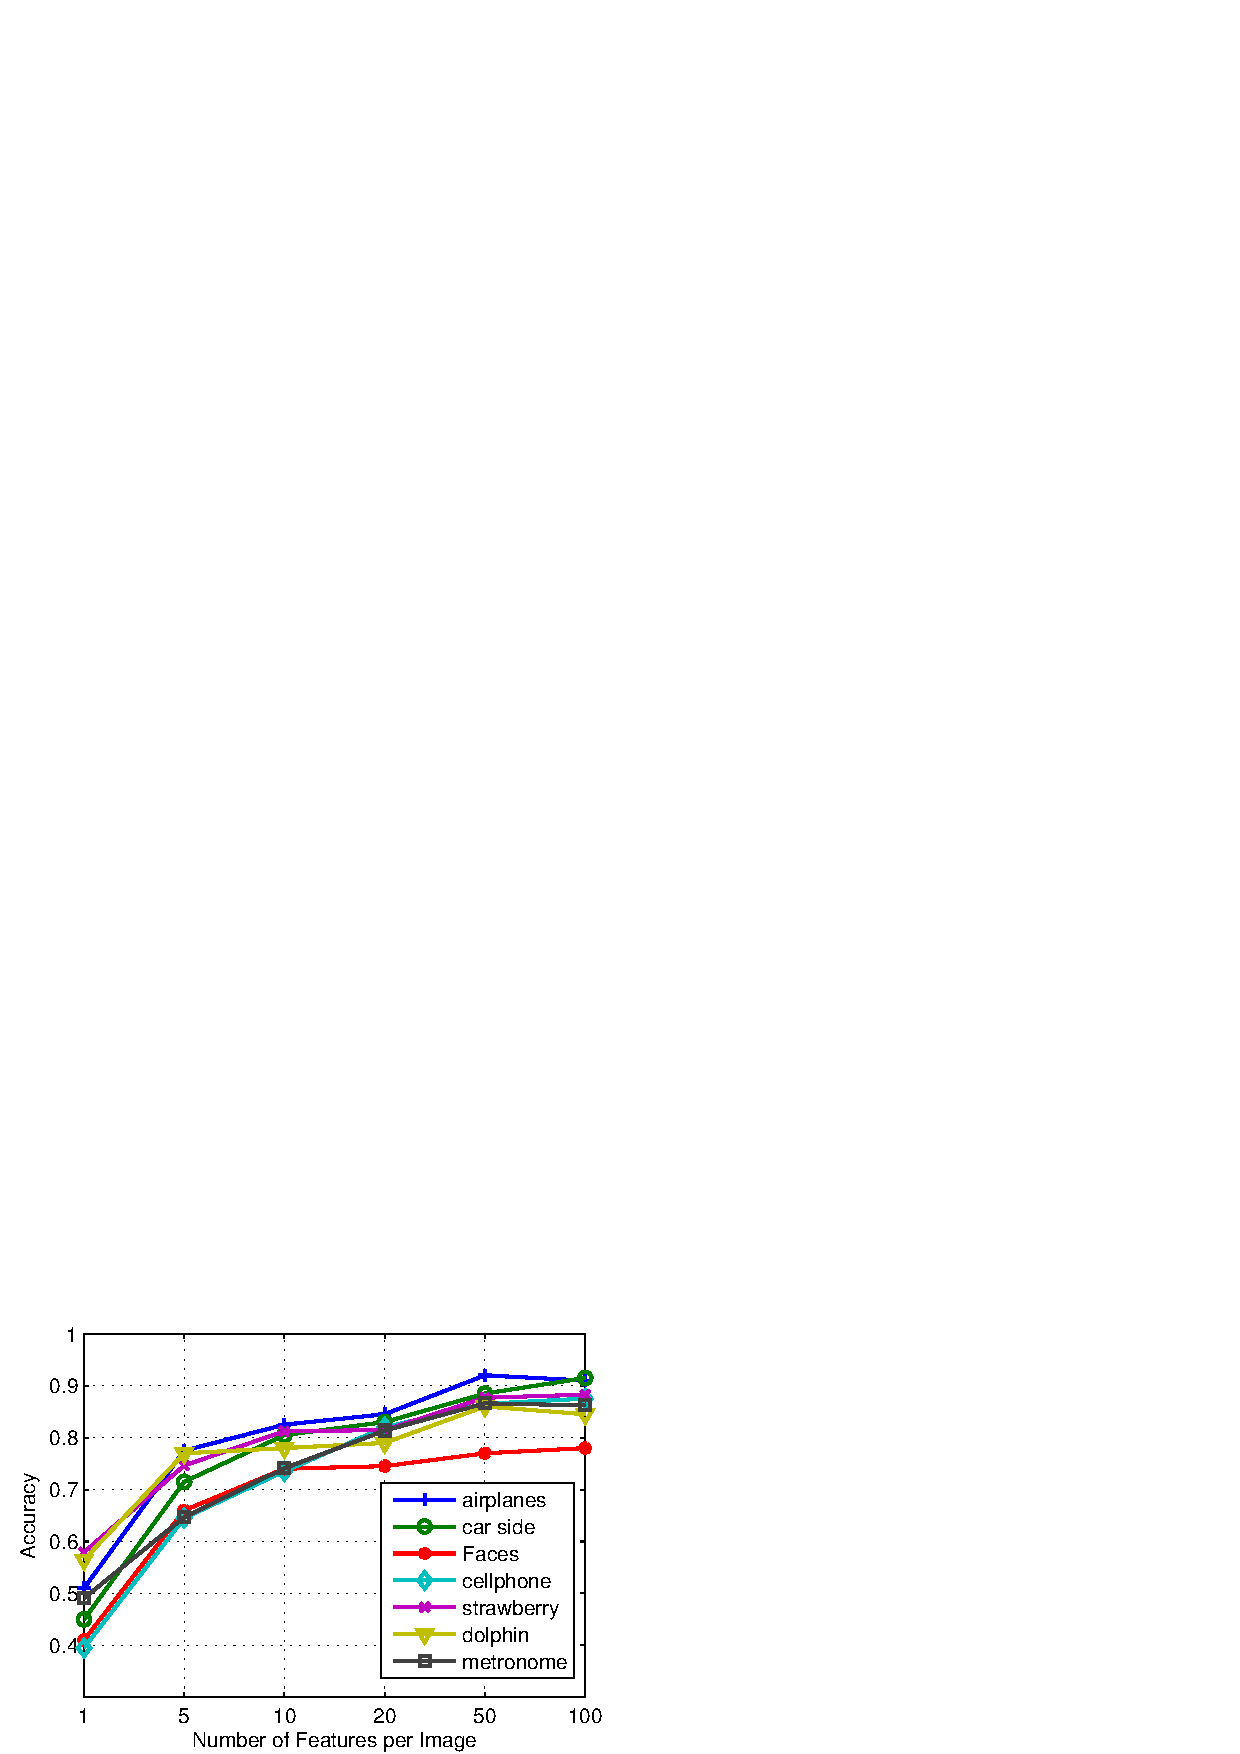
\includegraphics[width=0.9\linewidth]{images/fig-15b.pdf}
    \label{fig:15b}}
\caption{Comparison of performance.}
\label{fig:15}
\end{figure}

\figurename~\ref{fig:15b} shows
the performance of our model over the 101 categories
compared with SIFT features \cite{lowe1999},
PHOW features \cite{lazebnik2006},
and biologically inspired HMAX model \cite{serre2007}.
The results are obtained with 30 training images randomly selected 
from each category.
SIFT features and neural features generated with our model
are passed to an SVM classifier.
The images passed to the HMAX model are resized 
to a uniform height of 140 pixels as recommended by \cite{serre2007}.
Our model exhibits competitive performance 
compared with other models.
As shown in \figurename~\ref{fig:15b},
the SIFT performance points over the 101 categories
are almost completely to the left of the equivalent line.
The PHOW performance points spread through 
a wider range from $0.5$ to $1$ indicating 
the lack of robustness compared with our model.
Compared with the biologically inspired HMAX model,
our performance is also better for more than half
of the 101 categories.

\section{Conclusion}\label{sec:conclusion}

In this paper, we make an attempt 
to construct a multi-layer neural network model 
that explicitly maps different layers 
to different stages in the visual pathway of object recognition. 
We demonstrate in experiments that local image features 
generated by this neural model show competitive performance 
in object discrimination. 
More over, this model provides a framework 
to take into account higher-level stages in visual processing, 
such as the area V4 and the IT cortex, 
and emulates object recognition mechanisms in the cortex.

There are at least two directions that could be
followed to further improve the model.
First, feedback connections should be
adopted for the reason that feedback connections
occur widely in the neural systems in the forms 
of both intra-layer and inter-layer feedbacks.
Second, computational units that better 
conform to the neural response patterns should
be well evaluated and adopted 
to replace the current coarse implementation 
of the V4 and IT layers.

\section*{References}

\bibliography{ref}

\end{document}